\subsection{Wybór komputera wyświetlającego obraz na ekranie}
\label{sec:Komputer wyświetlający obraz na ekranie}

Klient to komputer podłączony bezpośrednio do ekranu wyświetlającego obraz. Istotnymi cechami takiego urządzenia są przede wszystkim:
\begin{itemize}
	\item niska cena
	\item wystarczająca moc obliczeniowa do uruchomienia przeglądarki, oraz prostej gry w technologi Flash, lub HTML5
	\item duża dostępność
	\item mały rozmiar
\end{itemize}

Głównym zadaniem klientów jest komunikacja serwerem poprzez sieć Ethernet w celu wyświetlania obrazu na podłączonym do klienta ekranie, oraz możliwość sterowania urządzeniami wejścia (klawiatura, myszka) poprzez udostępniony interfejs w sieci Ethernet.

Jeśli chodzi o wybór architektury procesora wybór był całkiem prosty, za sprawą sporej liczby dostępnych urządzeń dostępnych w tej architekturze (32 bitowa architektura ARM\footnote{Advanced RISC Machine} jest najczęściej stosowaną architekturą w urządzeniach mobilnych\cite{acm}), jak i uzasadnioną ich popularnością. Architektura ARM cechuje cię niskim poborem energii, dużą niezawodnością w systemach wbudowanych, oraz dla praktycznie wszystkich dostępnych na rynku procesorów możliwością instalacji w pełni funkcjonalnego systemu operacyjnego.
Procesory oparte o architekturę ARM przetwarzają instrukcje z wykorzystaniem mechanizmu potokowania. Procesor może wykonywać trzy rodzaje instrukcji:
\begin{itemize}
	\item 32-bitowe ARM
	\item 64-bitowe ARM (Apple A7)
	\item 16-bitowe Thumb (oraz Thumb2)
\end{itemize}

\par
Firma ARM projektuje rdzenie procesorów i sprzedaje je producentom. Producenci z kolei tworzą urządzenia typu SoC \footnote{ang. \emph{System on Chip} scalony system mikroprocesorowy często wyposażony w dodatkowe bloki funkcyjne, jednostki wektorowe czy procesory sygnałowe}. Istnieje też spora lista firm, które projektują swoje rdzenie wykorzystujące zbiór instrukcji ARM m.in. Apple, XScale, czy Faraday.

\par
Istotną cechą, którą powinien posiadać procesor ARM jest jednostka MMU\footnote{Memory Managment Unit}. Jest to jednostka odpowiadająca za dostęp do zewnętrznej pamięci, translacje adresu wirtualnego na fizyczny, oraz kontroli uprawnień dostępu do pamięci. Wiele rdzeni ARM nie jest wyposażonych w tą jednostkę, która staje się obligatoryjna podczas gdy chcemy zainstalować system operacyjny Linux. 
\par

Po wyborze architektury procesora należy wybrać rodzinę procesora. Rodzina Cortex jest kolejną generacją procesorów po ARM7, ARM9, czy ARM11.

\begin{figure}
\begin{center}
	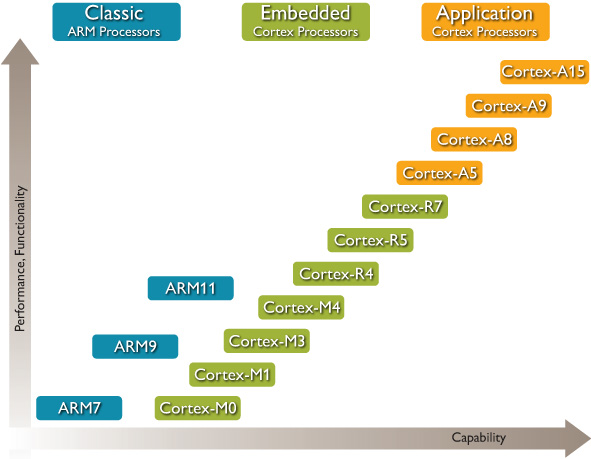
\includegraphics[scale=0.6]{ARM_Comparison}
\end{center}
\caption{Porównanie rodzin architektury ARM}
\label{fig:ARM_Comp}
\end{figure}

Zgodnie z tym co można zauważyć na rysunku~\ref{fig:ARM_Comp} architektura Cortex jest rodziną cechującą się wyższym od swoich poprzedników współczynnikiem wydajności na cykl zegara i niższym zużyciem energii.

Na rynku można wyodrębnić 3 główne chipy bazujące na architekturze ARM:
\begin{itemize}
	\item Allwinner (sunxi)
	Przykładowe produkty:
	\begin{itemize}
		\item Hackberry A10
		\item MK802
	\end{itemize}

	Chipy Allwinnera charakteryzują się stosunkowo najniższą ceną, oba przedstawione wyżej modele bazują na rdzeniu Cortex-A8 taktowane zegarem 1GHz, oraz dysponujące 1GB pamięci operacyjnej. Wyposażone są także w procesor graficzny ARM Mali 400
	
	\item Freescale i.MX6 (imx)
	Przykładowe produkty:
	\begin{itemize}
		\item MarS
		\item IMX53QSB
	\end{itemize}
	\item TI OMAP3/4
	Przykładowe produkty:
		\begin{itemize}
			\item Beaglebone Black
			\item Panda Board
		\end{itemize}
	Ta rodzina zyskała bardzo dużą popularność. Chipy OMAP3 wyposażone są w zmiennoprzecinkową jednostkę oraz zestaw instrukcji wektorowych NEON. Główną cechą tego rozwiązania jest dużo wydajność operacji przy zachowaniu prostoty ich programowania.
\end{itemize}

\subsection{System operacyjny dla komputera wyświetlającego obraz na ekranie.}

Nie dysponując zbyt dużą mocą obliczeniową, małą pamięcią operacyjną, oraz niewielką przestrzenią dyskową należy dobrze dobrać, oraz skonfigurować system operacyjny. Do tego celu wybrano dystrybucje linuksa - Debian. Cechuje się ona przede wszystkim wysoką stabilnością (bardzo często wybierana jako system serwerowy), oraz sporą społecznością programistów rozwijających tą dystrybucje co przekłada się na mnogość dostępnych pakietów przygotowanych specjalnie dla tej wersji systemu Linux. Wreszcie system Debian jest wysoce konfigurowalny - oparty o jądro Linux, daje użytkownikowi możliwość zbudowania systemu od podstaw. Dlatego też jako system docelowy i główny, wybraliśmy dystrybucje Debian.

\begin{figure}
\begin{center}
    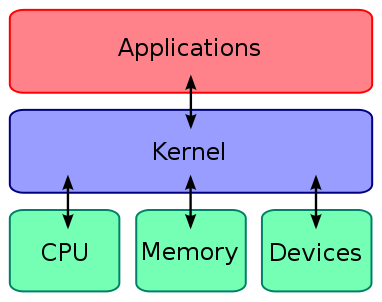
\includegraphics[scale=0.5]{kernel}
\end{center}
\caption{Działanie jądra systemu Linux}
\label{fig:kernel}
\end{figure}

Jądro \footnote{ang. \emph{Kernel}} systemu Linux jest centralnym miejscem systemu operacyjnego. Jak zaprezentowano na rysunku ~\ref{fig:kernel} jest ono najniżej usytuowaną warstwą systemu operacyjnego odpowiadającą za komunikację z procesorem, pamięcią, czy urządzeniami zewnętrznymi. Kernel m.in. przydziela odpowiednią ilość pamięci operacyjnej dla każdej aplikacji, obsługuje komunikaty i komunikacje między procesorową.

Pierwotnym twórcą jądra Linux jest programista pochodzenia duńskiego Linus Torvalds, natomiast obecnie jądro systemu Linux jest rozwijane przez programistów z całego świata. Jego aktualną wersje można pobrać z oficjalnego otwartego repozytorium github.






